\chapter{Results}\label{chap:results}

\section{Total energy as a function of time for different time steps}
    \graphicspath{ {./figures/milestone04/} }
    \begin{figure}[!htb]
    % \captionsetup{justification=centering,margin=2cm}
    \centering
        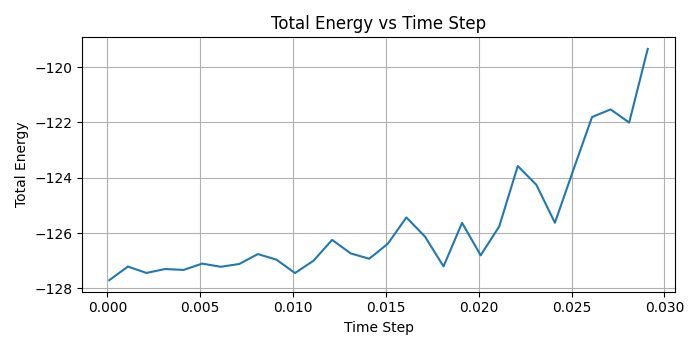
\includegraphics[scale=0.9]{total_energy_vs_time_step.png}
        \caption[Total energy vs Time steps using parameters]{\textbf{Total energy vs Time steps using parameters: start\_time\_step=1e-4, end\_time\_step=30e-3,step=1e-3, sigma=1, mass=1, epsilon=1, total\_time=5000}}
    \label{fig:total_energy_vs_time_step}
    \end{figure}
As we increase the time step the total energy of the system increases and at some point the system becomes unstable and the atoms start to move away from each other
and the simulation stops. This is because the time step is too large and the atoms are not able to move to the correct position in the next time step.


\section{Snapshots sequence of LJ simulation}
    \graphicspath{ {./figures/milestone04/} }
    \begin{figure}[h]

    \centering
        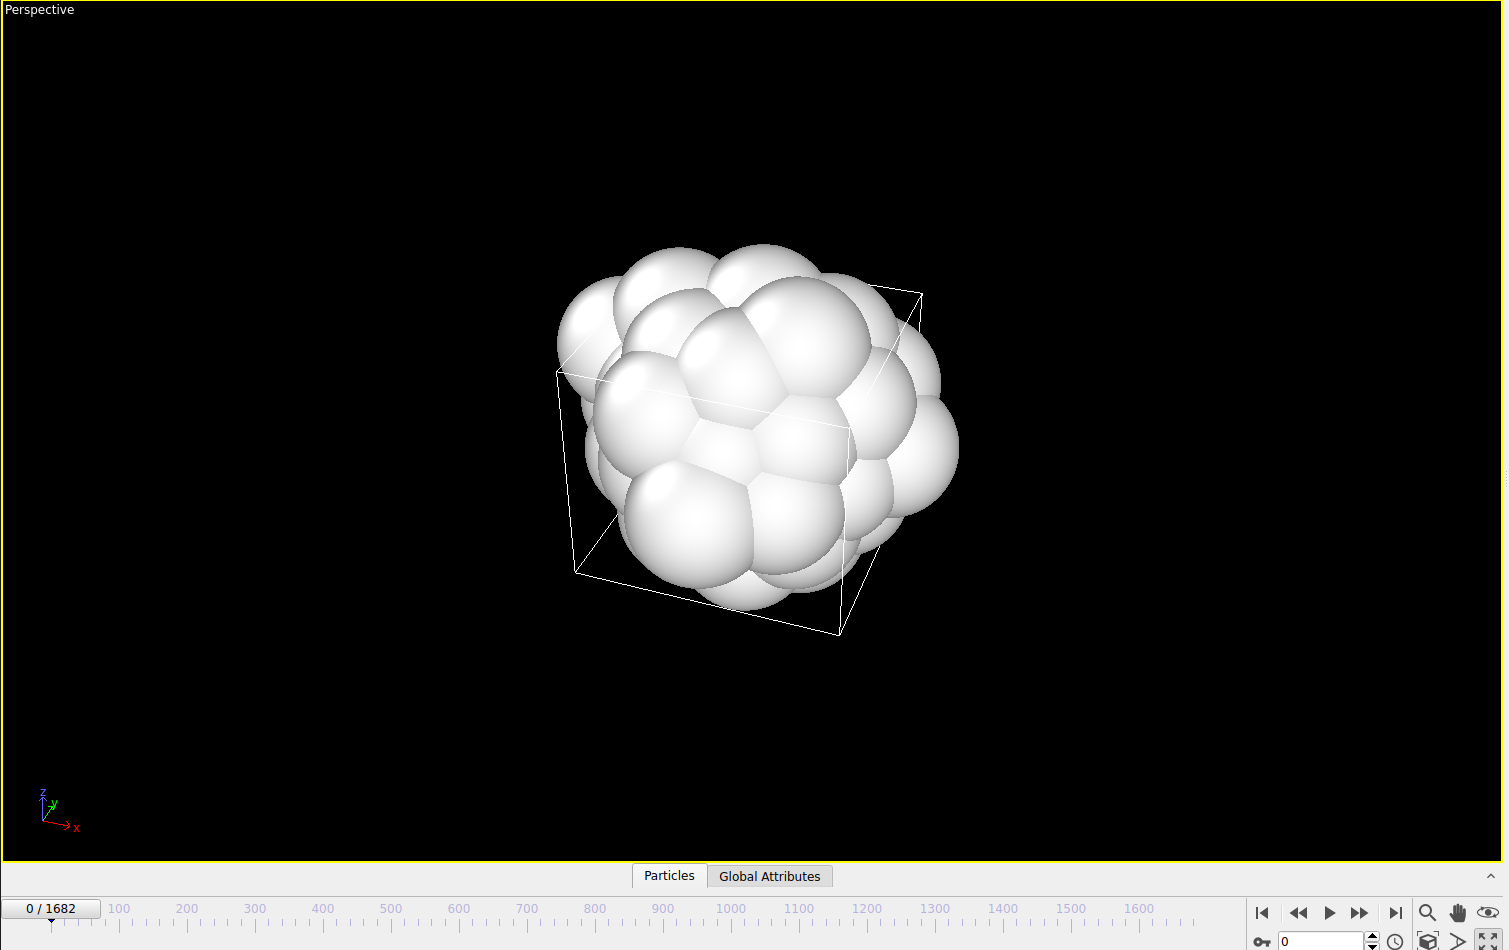
\includegraphics[scale=0.25]{ML1.png}
        \caption{LJ simulation snapshot1}
    \label{fig:step1}
    \end{figure}
    \begin{figure}[!htb]
    \centering
        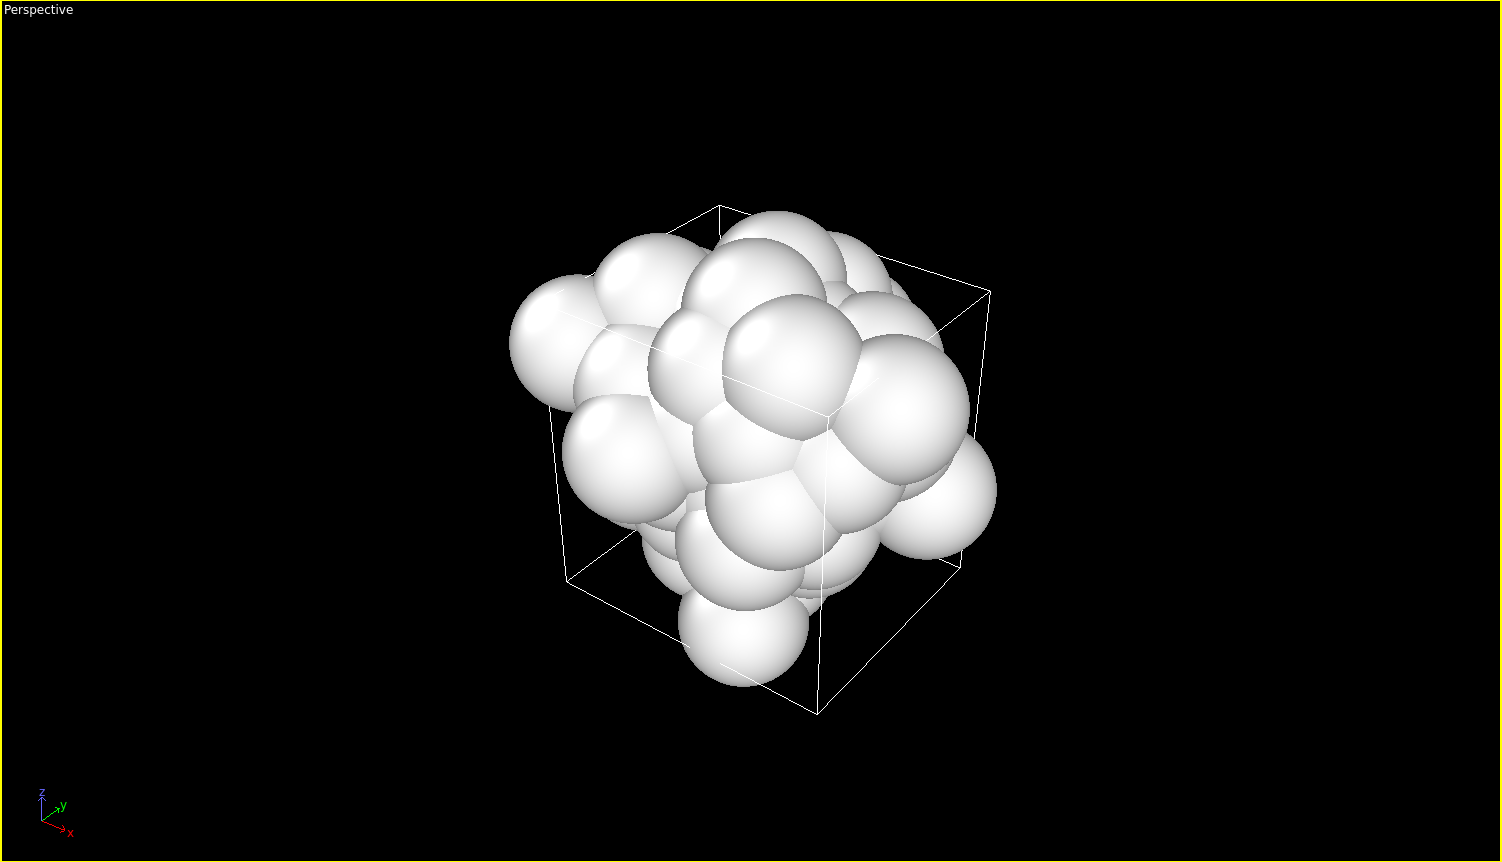
\includegraphics[scale=0.25]{ML2.png}
        \caption{LJ simulation snapshot2}
    \label{fig:step2}
    \end{figure}
    \begin{figure}[!htb]
    \centering
        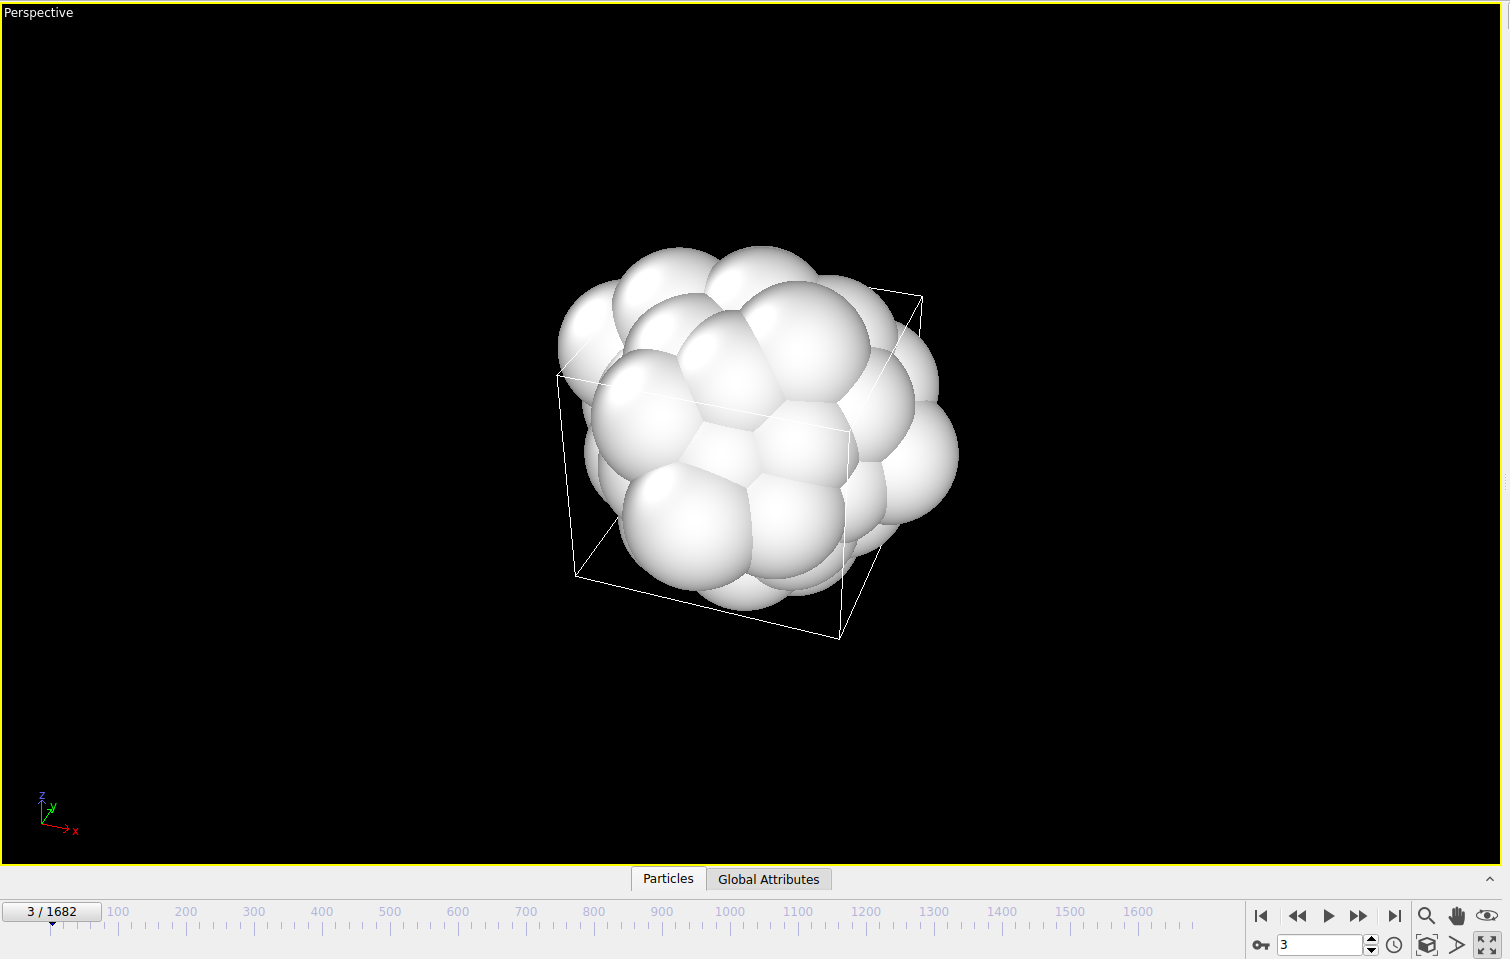
\includegraphics[scale=0.25]{ML3.png}
        \caption{LJ simulation snapshot3}
    \label{fig:step3}
    \end{figure}
    \begin{figure}[!htb]
    \centering
        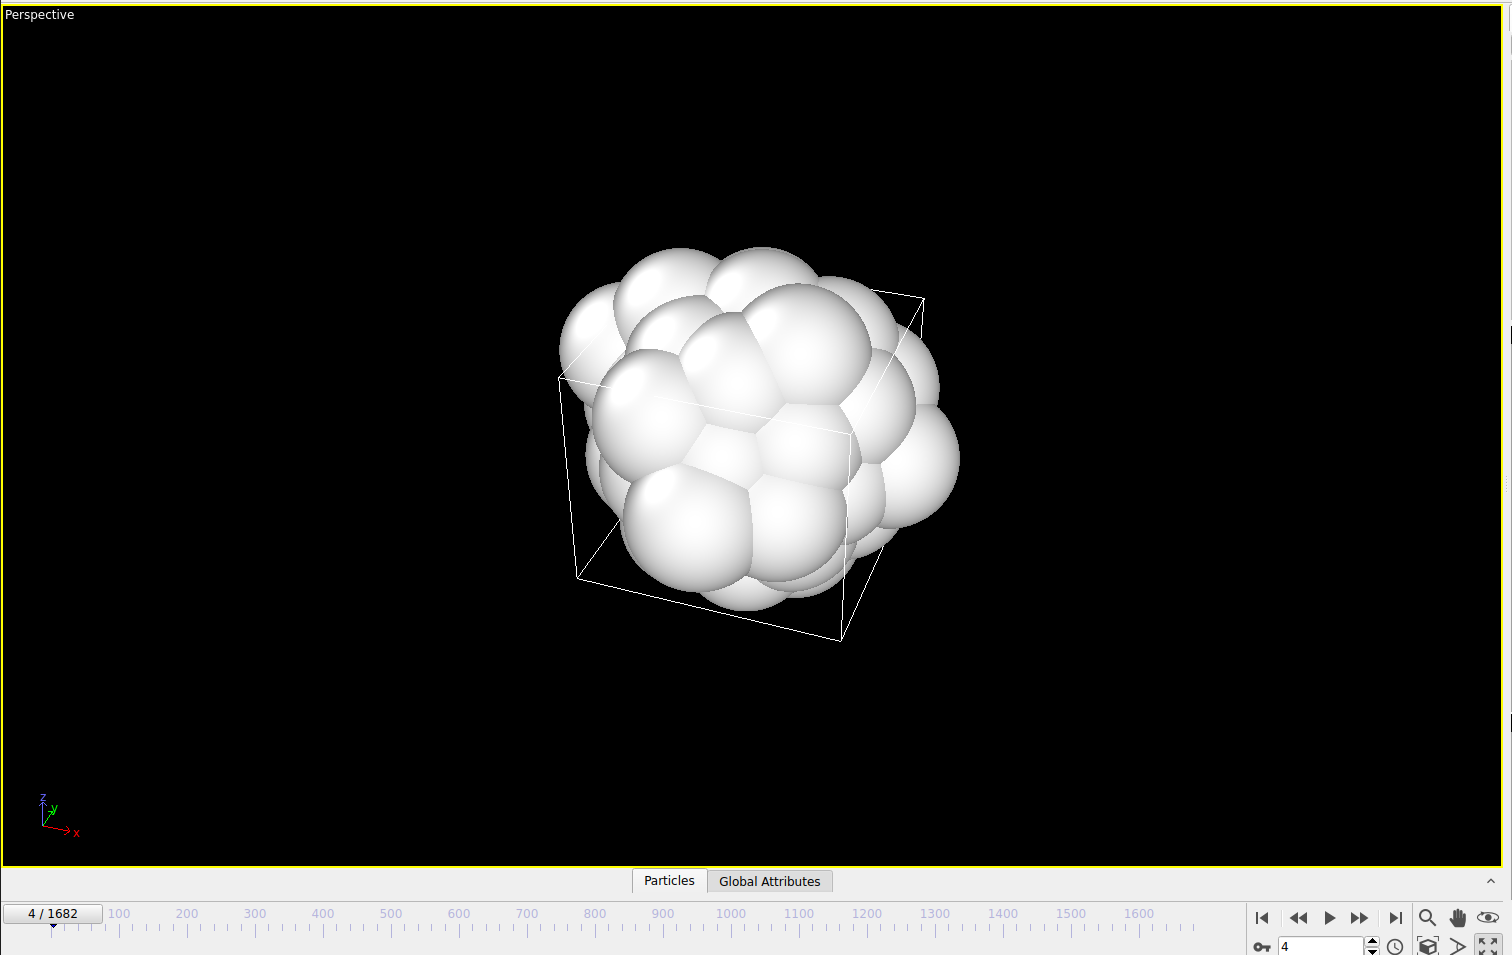
\includegraphics[scale=0.25]{ML4.png}
        \caption{LJ simulation snapshot4}
    \label{fig:step4}
    \end{figure}
    \begin{figure}[!htb]
    \centering
        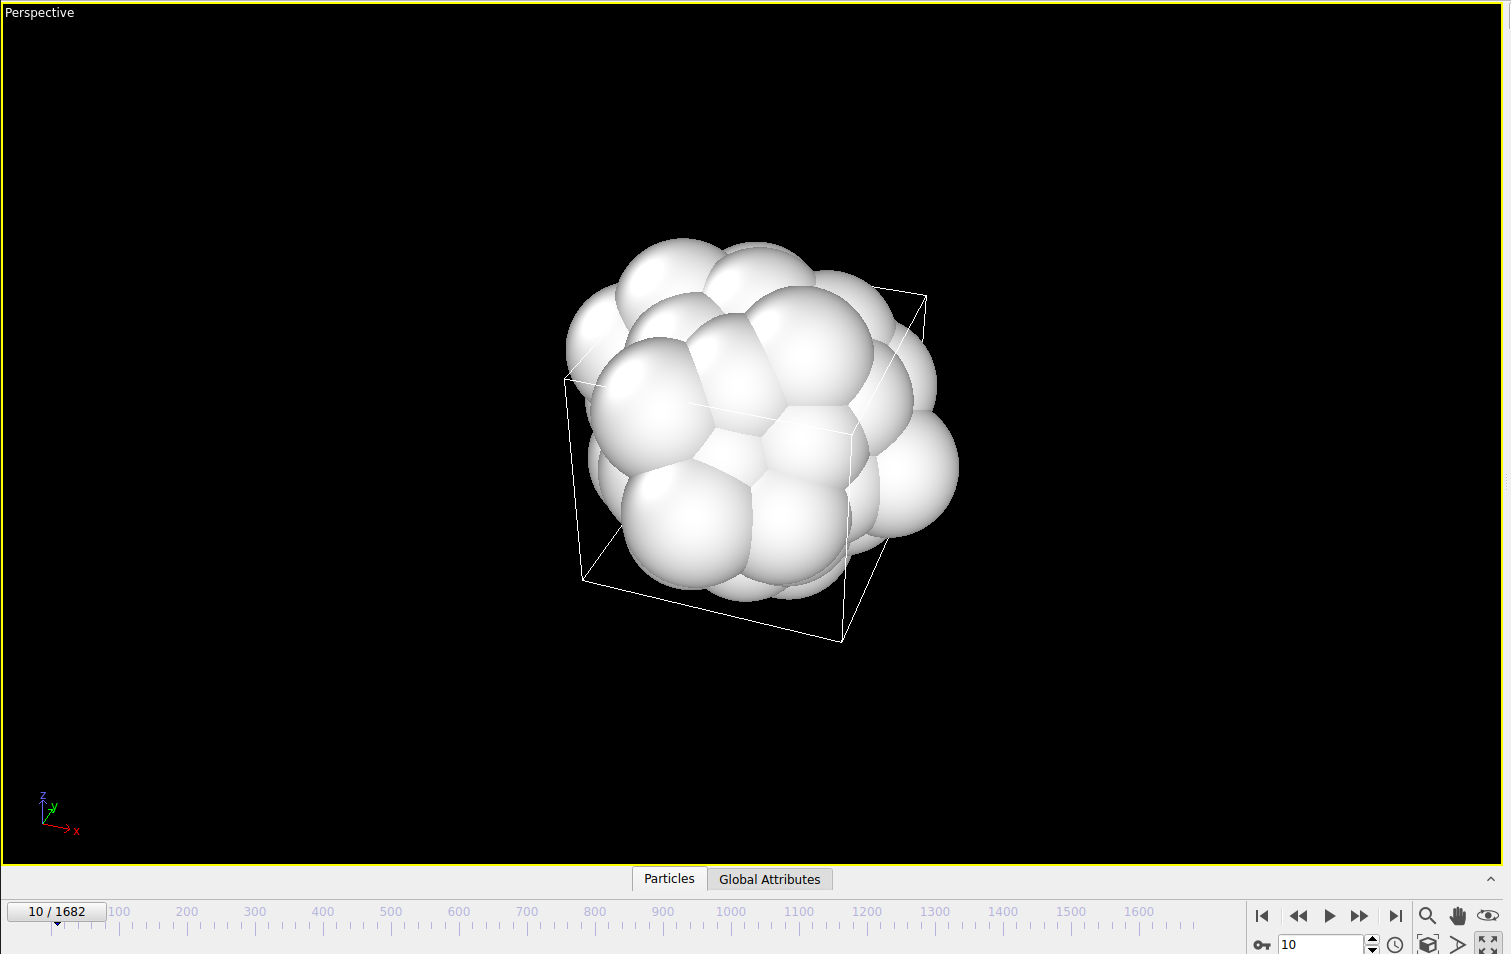
\includegraphics[scale=0.25]{ML5.png}
        \caption{LJ simulation snapshot5}
    \label{fig:step5}
    \end{figure}



\section{simulation time as a function of the size (number of atoms) without neighbor list}
    \graphicspath{ {./figures/milestone05/} }
    \begin{figure}[!htb]
    \centering
        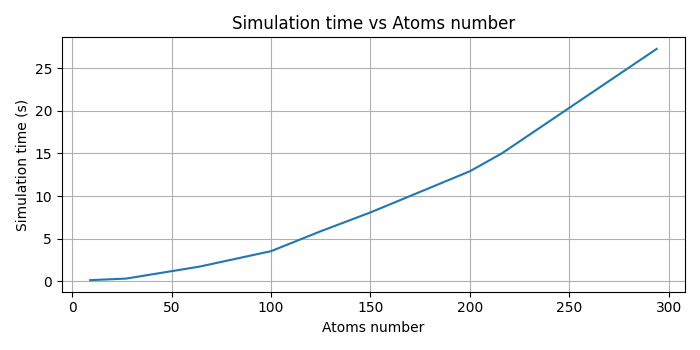
\includegraphics[scale=0.9]{simulation_time_vs_atoms_number.png}
        \caption[Simulation time vs Atoms number]{\textbf{Simulation time vs Atoms number using parameters: time\_step=1e-3, sigma=1, mass=1, epsilon=1, total\_time=5000, relaxation\_time\_start = 10* time\_step,then after reaching equilibrium, it increases to 50*time\_step.}}
    \label{fig:simulation_time_vs_atoms_number}
    \end{figure}
    Here we notice that the simulation time increases quadratically with the number of atoms in the system. This is because in the energy update step in the LJ simulation we have to calculate the energy between all the pairs of atoms in the system. So the time complexity of the energy update step is $O(N^2)$ where $N$ is the number of atoms in the system. For example, In the figure above,The  simulation time for 100 atoms is 3.5s and for 200 atoms is 12.9s which is almost 4 times more than the simulation time for 100 atoms.

\section{simulation time as a function of the size (number of atoms) with neighbor list}
    \graphicspath{ {./figures/milestone06/} }
    \begin{figure}[!htb]
    \centering
        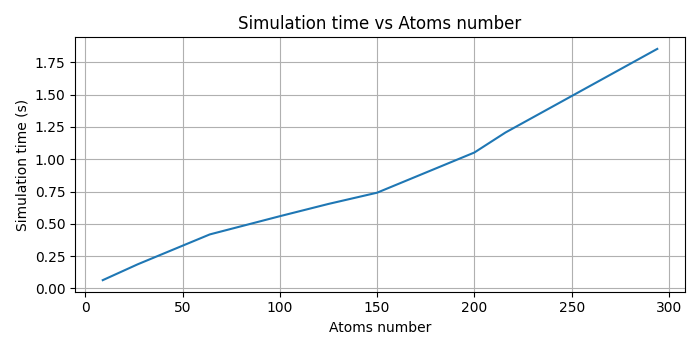
\includegraphics[scale=0.9]{simulation_time_vs_atoms_number.png}
        \caption[Simulation time vs Atoms number]{\textbf{Simulation time vs Atoms number using parameters: time\_step=1e-3, sigma=1, mass=1, epsilon=1, total\_time=5000, relaxation\_time\_start = 10* time\_step,then after reaching equilibrium, it increases to 50*time\_step, and cutoff\_radius = 1.5.}}
    \label{fig:simulation_time_vs_atoms_number}
    \end{figure}
    Here, it's very clear the linearity of the simulation time with the number of atoms in the system. By introducing the concept of just calculating the energy between the atoms that are close to each other, we have reduced the time complexity of the energy update step from $O(N^2)$ to $O(N)$ where $N$ is the number of atoms in the system. For example, In the figure above,The  simulation time for 100 atoms is 0.56s and for 200 atoms is 1.05s which is almost 2 times more than the simulation time for 100 atoms.

\section{total energy vs temperature}
The setup for this section is as follows:
    \begin{itemize}
        \item time\_step=1fs
        \item mass=20405.7294 amu
        \item relaxation\_time\_start = 10* time\_step,then after 500 step, it increases to 1e10*time\_step
        \item cutoff\_radius = 10 Angstrom
        \item added\_energy\_in\_each\_experiment=0.01*no\_atoms
        \item atomic\_distance = 2.885
        \item cluster\_sizes=3:12
        \item for cluster sizes 3:8 
        \subitem  target\_temp = 300 K
        \subitem  initial\_simulation\_time=10000fs
        \subitem  experiment\_simulation\_time=5000fs
        \subitem  number\_experiments=26
        \item for cluster sizes 9:12 
        \subitem  target\_temp = 500 K
        \subitem  initial\_simulation\_time=5000fs
        \subitem  experiment\_simulation\_time=2000fs
        \subitem  number\_experiments=40
    \end{itemize}
    \graphicspath{ {./figures/milestone07/} }
    \begin{figure}[!htb]
    \centering
        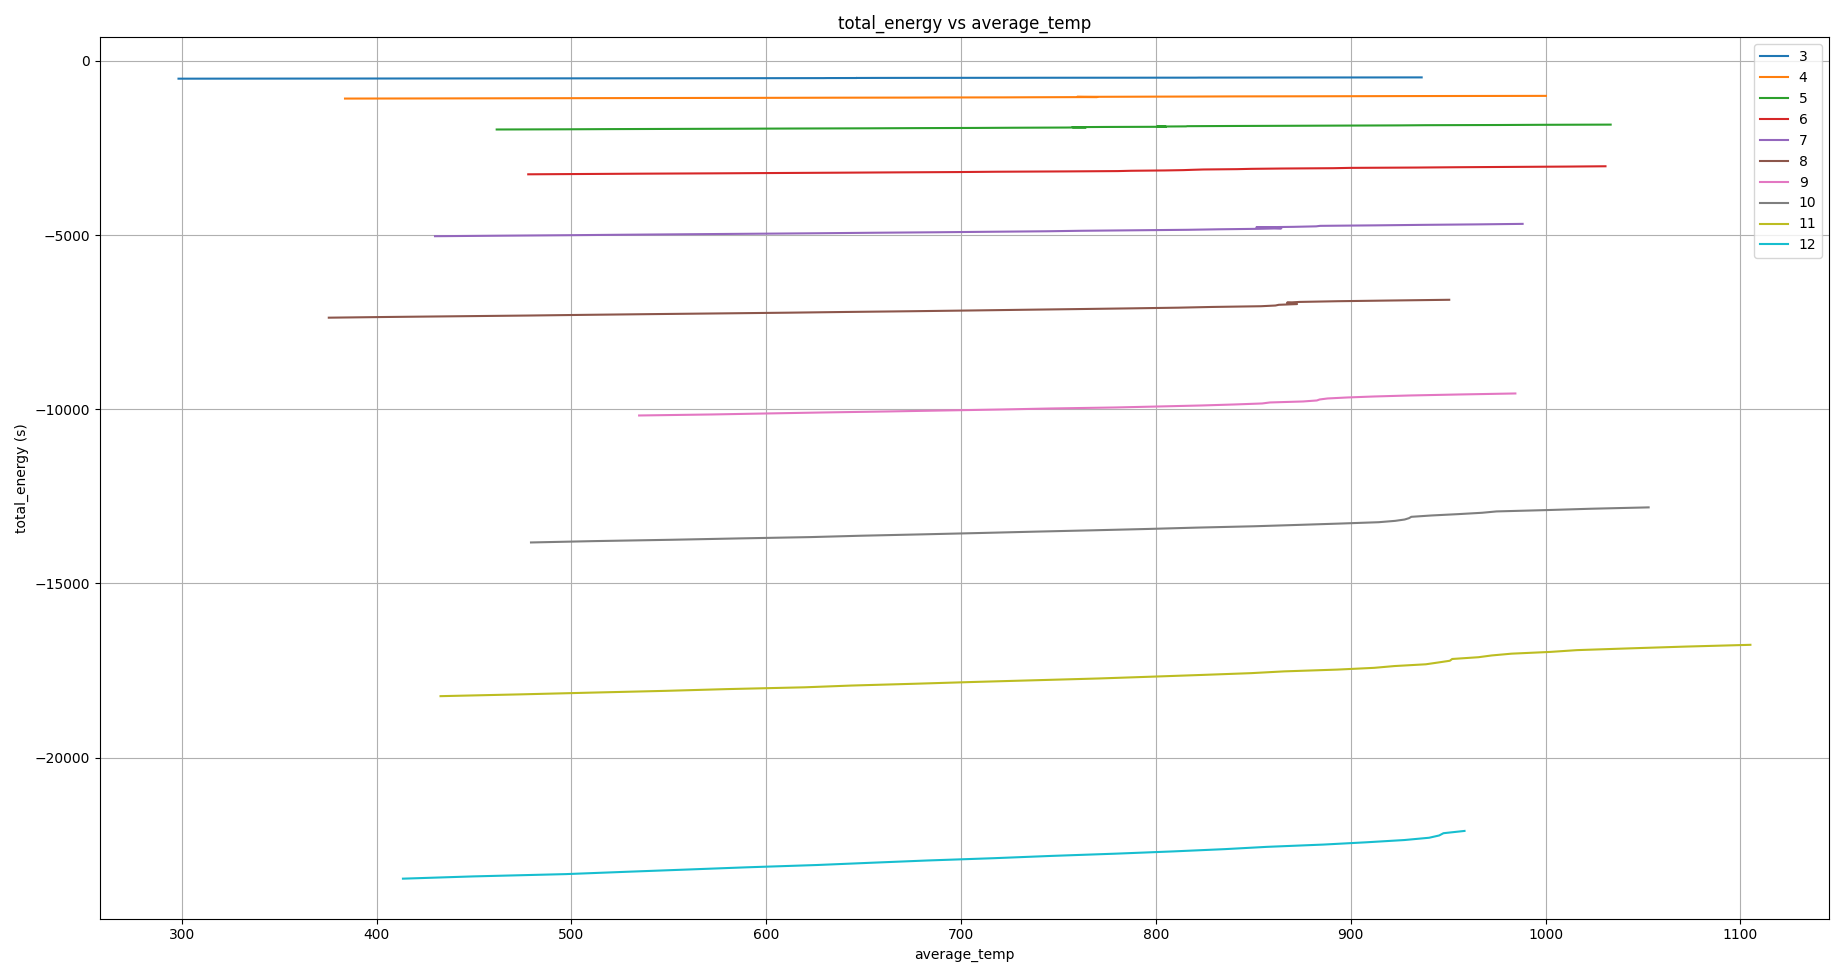
\includegraphics[scale=0.35]{total_energy_vs_average_temp.png}
        \caption{Total energy vs Temp}
    \label{fig:simulation_time_vs_atoms_number}
    \end{figure}
    As the temperature increases the total energy of the system increases. This is because the atoms are moving faster and they are colliding with each other more often. This leads to more energy being transferred between the atoms and the total energy of the system increases. The total energy of the system is conserved and it is equal to the sum of the kinetic energy of the atoms and the potential energy between the atoms. So as the temperature increases the kinetic energy of the atoms increases and the potential energy between the atoms decreases. This is why the total energy of the system increases as the temperature increases.  

    Near the melting point we notice that Adding more energy to the system doesn't increase the total energy of the system anymore but instead it decreases the total energy of the system. This is because the atoms are not able to absorb the energy and the system is in equilibrium. So the atoms are vibrating around their equilibrium position and the energy is being transferred between the atoms and the total energy of the system decreases.

\section{melting point versus cluster size}
    The setup for this section is the same as the one used in the previous section.
    \graphicspath{ {./figures/milestone07/} }
    \begin{figure}[!htb]
    \centering
        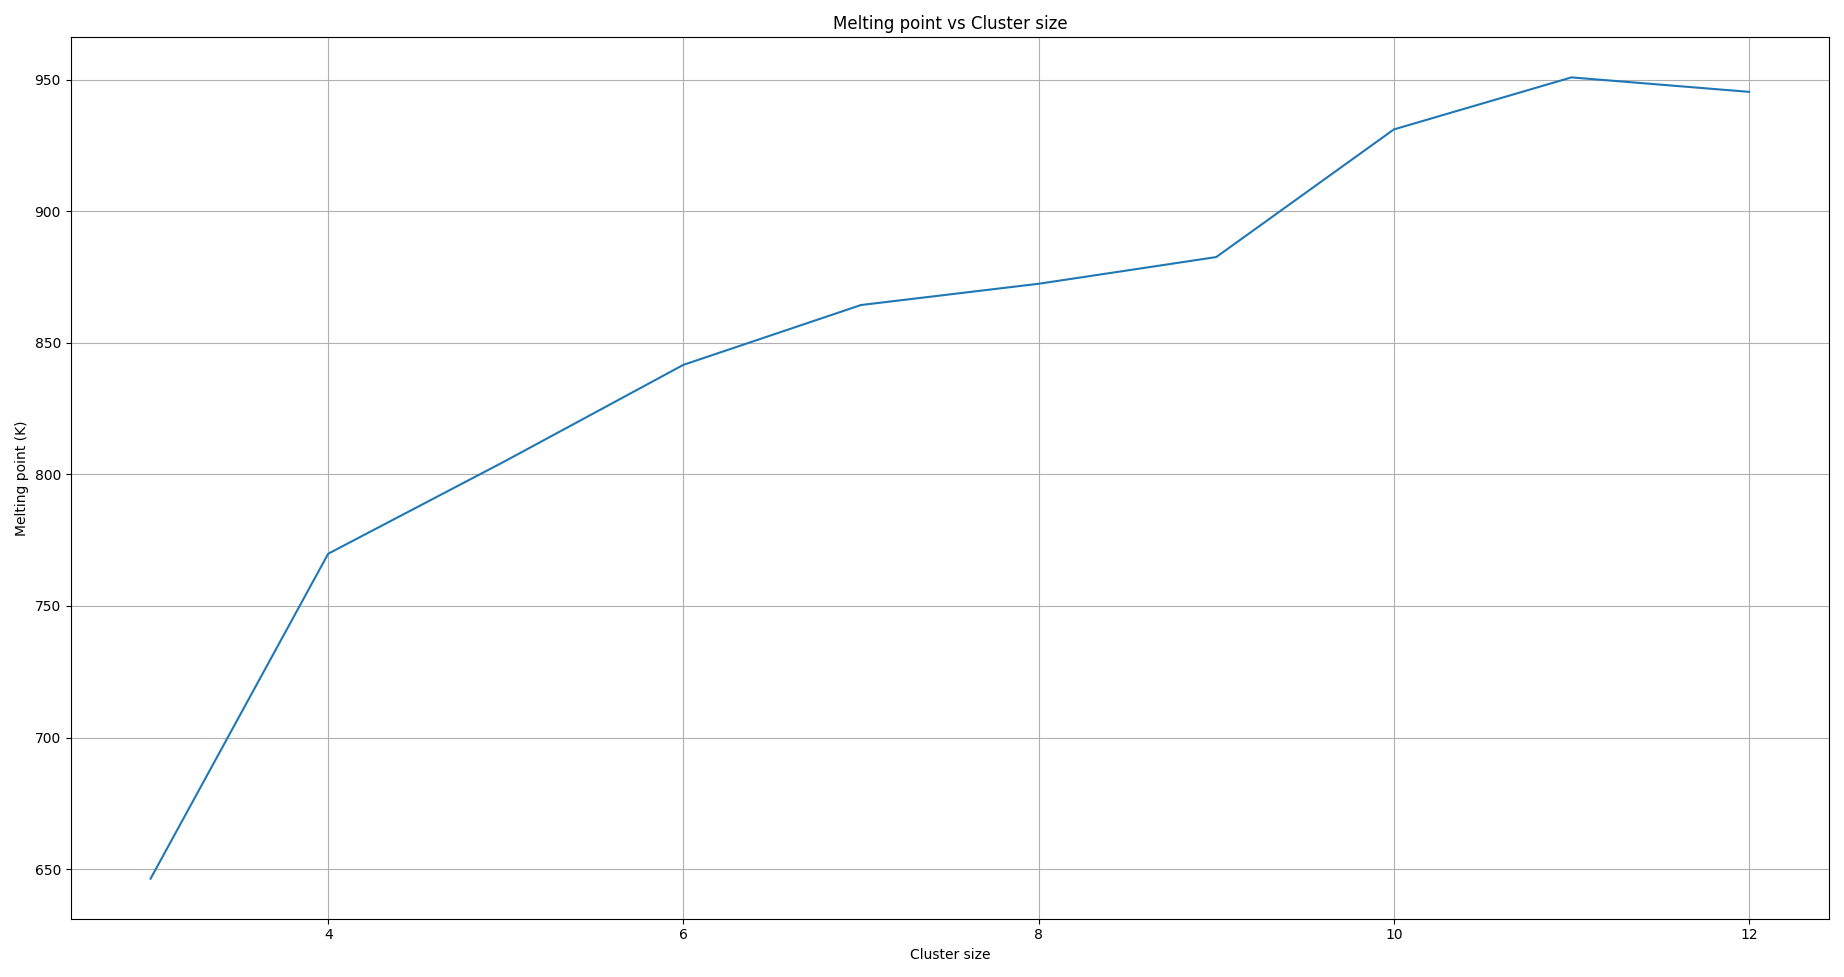
\includegraphics[scale=0.35]
        {melting_point_vs_cluster_size.png}
        \caption{Melting point vs cluster size}
    \end{figure}
    Here, as the cluster size increases the melting point increases because to melt a bigger cluster of atoms we need to add more energy to the system. This is because the atoms in the bigger cluster are more tightly packed and they are more difficult to melt.

\section{heat capacity versus cluster size}
    The setup for this section is the same as the one used in the previous section.
    \graphicspath{ {./figures/milestone07/} }
    \begin{figure}[!htb]
    \centering
        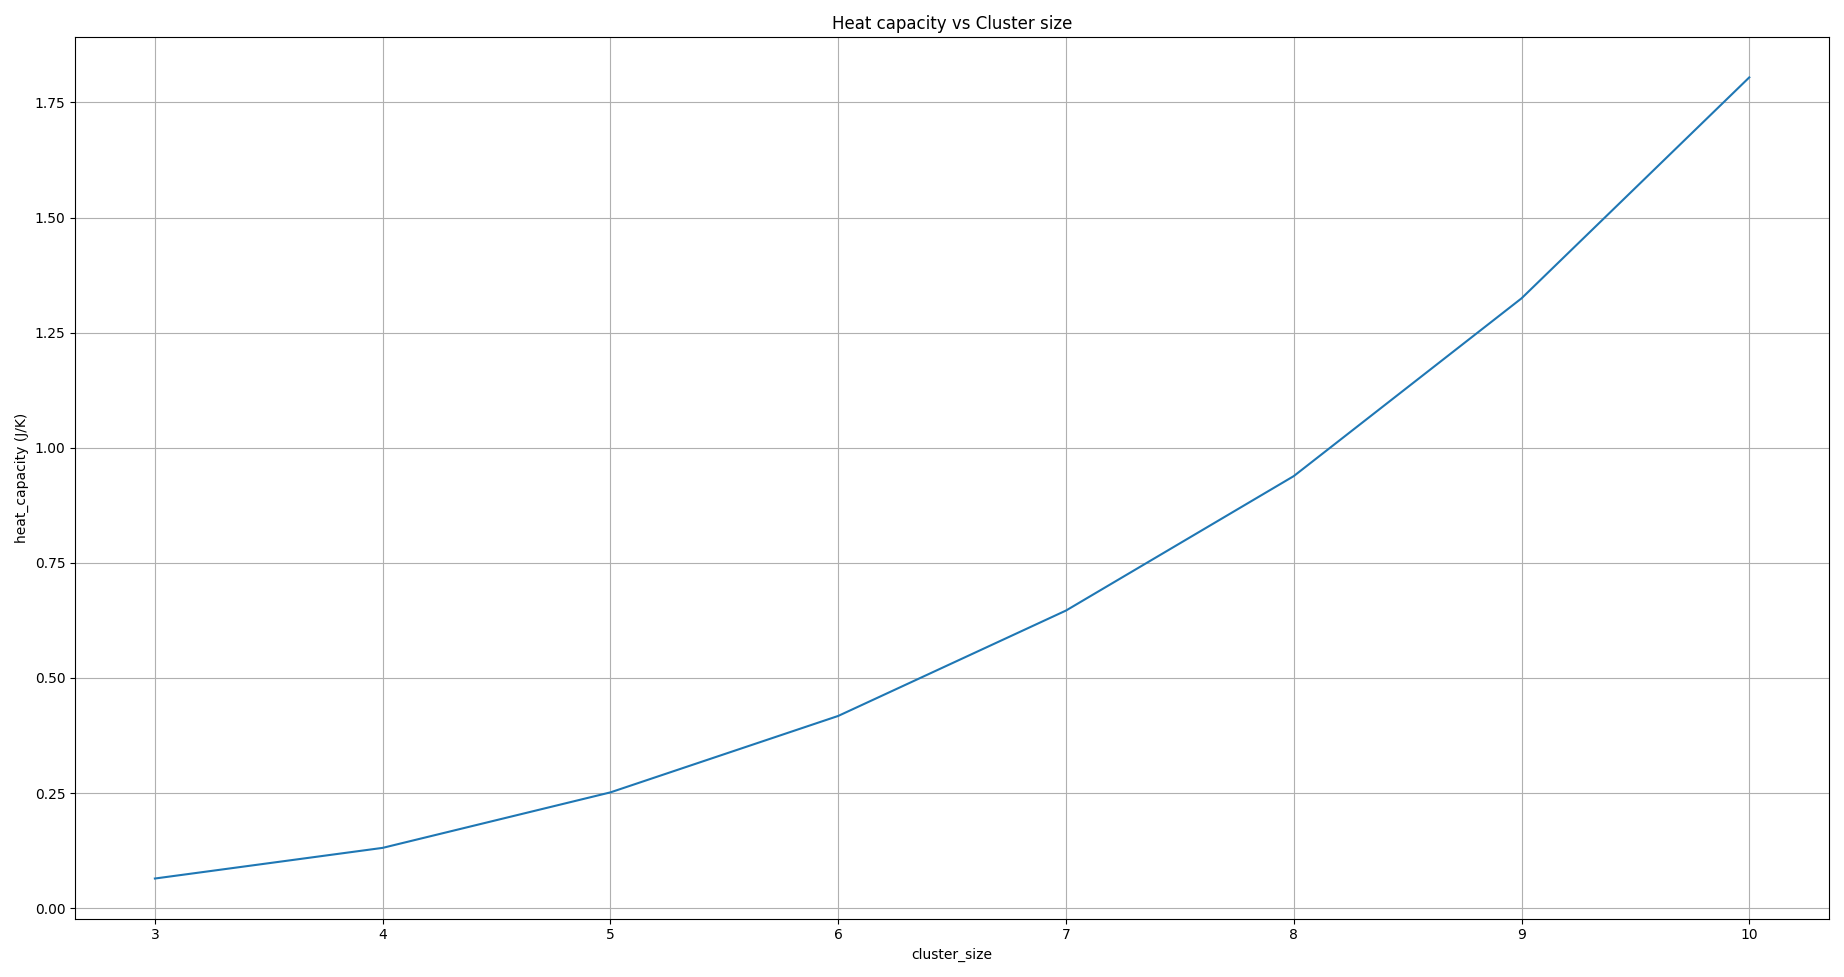
\includegraphics[scale=0.35]{heat_capacity_vs_cluster_size.png}
        \caption{Heat capacity vs cluster size}
    \end{figure}
    Here, as the cluster size increases the heat capacity increases.

\section{latent heat versus cluster size}
The setup for this section is the same as the one used in the previous section.
    \graphicspath{ {./figures/milestone07/} }
    \begin{figure}[!htb]
    \centering
        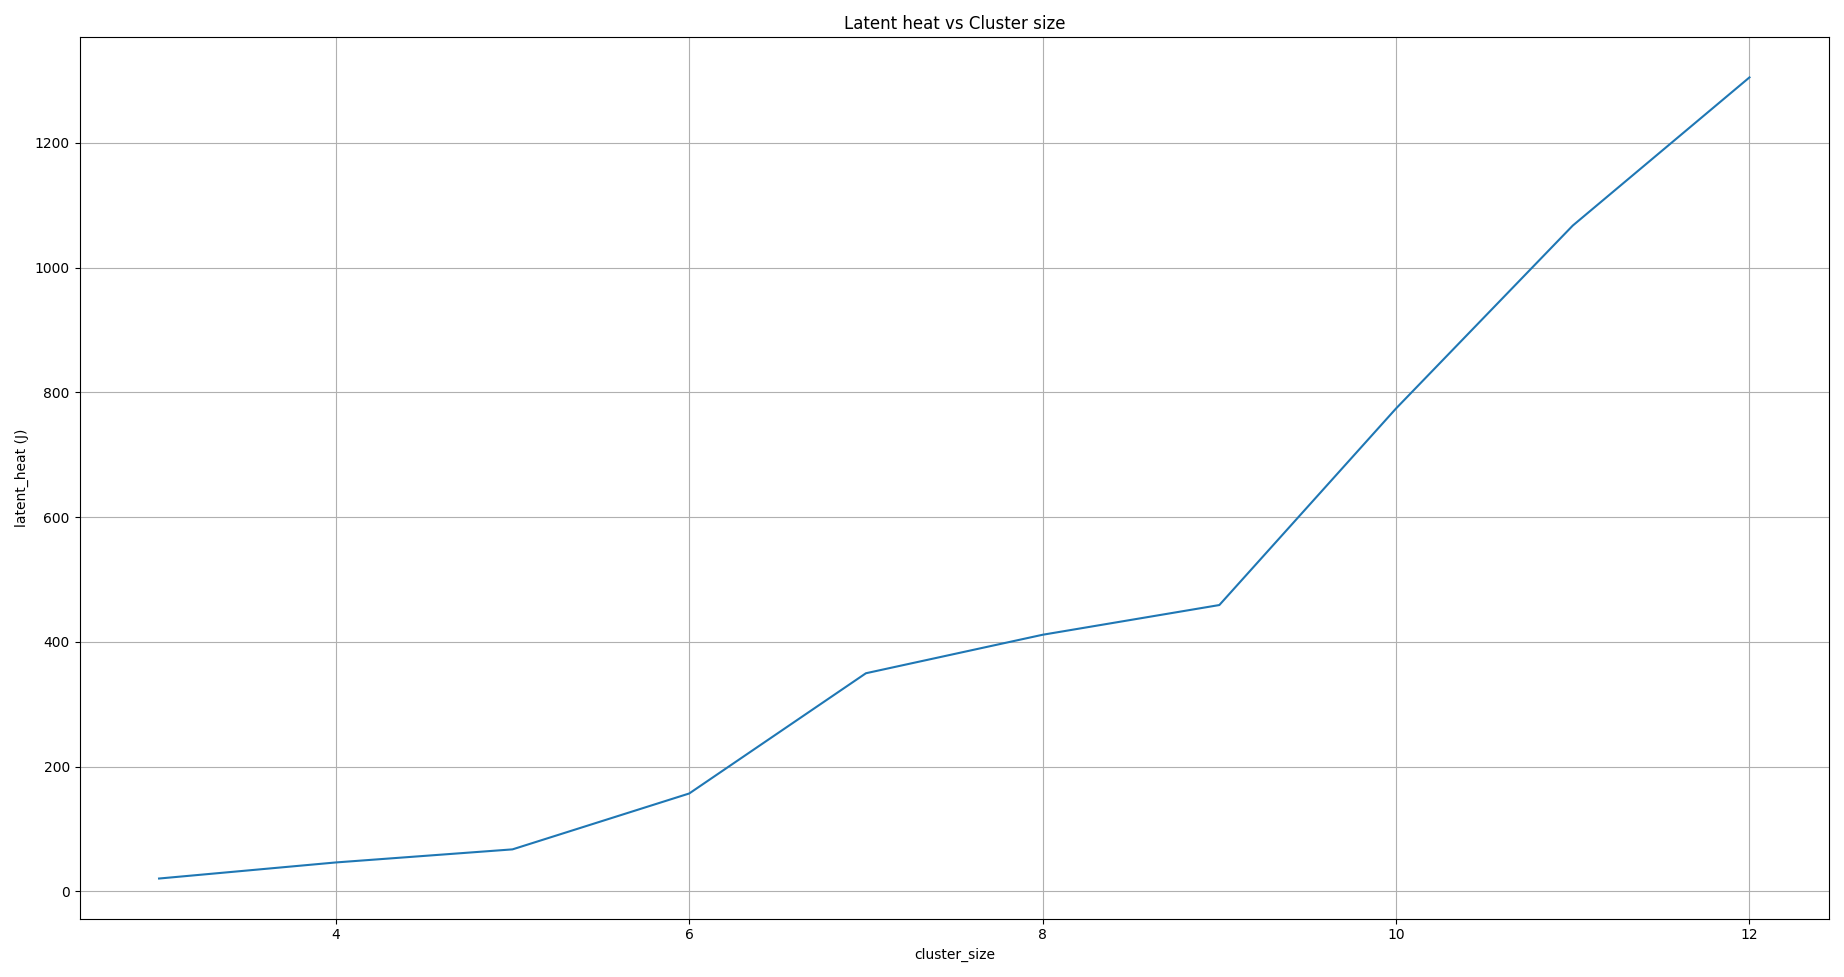
\includegraphics[scale=0.35]{latent_heat_vs_cluster_size.png}
        \caption{Latent heat vs cluster size}
    \end{figure}
    Here, as the cluster size increases the latent heat increases.


\section{Energy conservation with MPI parallelization}
% \section{Nanowire σ/ɛ}
\section{Nanowire defects}